\chapter{刚体定轴转动}
\setcounter{example_counter}{1}

\section{刚体转动的描述}

\subsection{刚体}

\textbf{刚体}是受力时形状和大小不发生改变的物体，是一种理想模型。

\subsection{刚体转动的描述}

对于刚体的定轴转动，我们只关心其转过的角度，因此可用角位移$\theta$、角速度$\omega$、角加速度$\alpha$描述，它们的关系与圆周运动的质点相同。

\begin{figure}[htb]
    \centering
    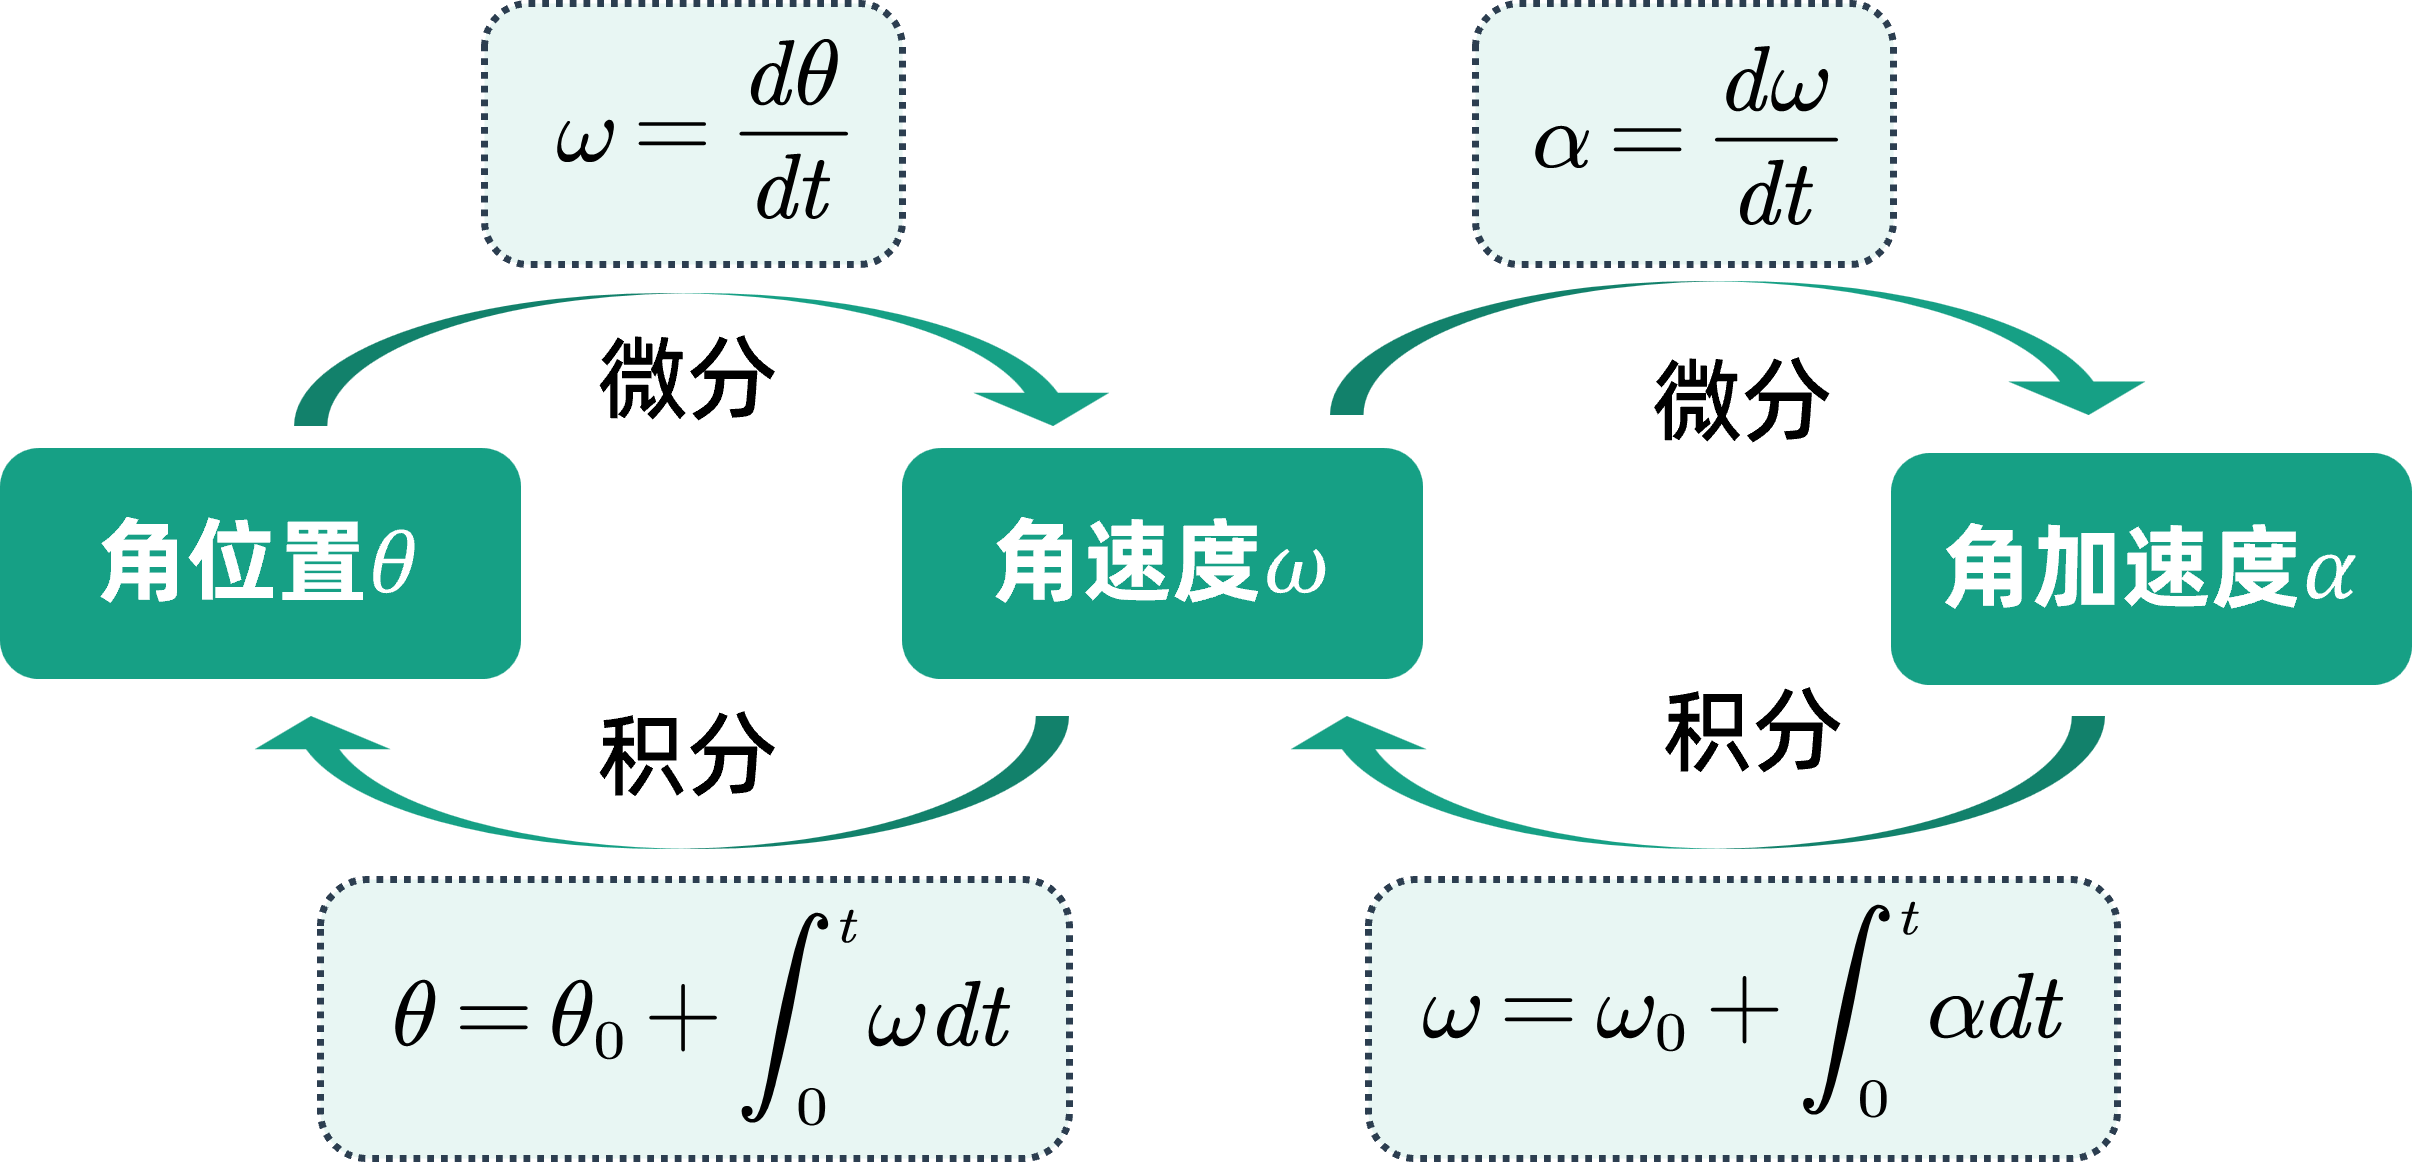
\includegraphics[width=0.6\linewidth]{asset/ch1/T8.png}
\end{figure}

\begin{formula}
    $\omega=\dfrac{d\theta}{dt},~\alpha=\dfrac{d\omega}{dt},~\theta=\theta_0+\displaystyle\int_0^t{\omega dt},~\omega=\omega_0+\displaystyle\int_0^t{\alpha dt}$
\end{formula}

\note{转动的角位移$\theta$、角速度$\omega$、角加速度$\alpha$的关系，与直线运动的位移$x$、速度$v$、加速度$a$的关系完全相同。}

\begin{example}{转动的描述}
    飞轮从$\SI{5}{rad/s}$开始均匀减速，在$\SI{20}{s}$后，角速度减为原来的$80\%$。求前$\SI{150}{s}$内转过的角度。
    \tcblower
    仿照匀变速直线运动的公式，把线量替换成角量，注意刹车陷阱。

    根据$\omega_1=\omega_0+\alpha t_1$，得角加速度$\alpha=\SI{-0.05}{rad/s^2}$，飞轮停下来的时间$t$满足$0=\omega_0+\alpha t_1$
    
    求得$t=\SI{100}{s}$，说明飞轮在$t=\SI{100}{s}$时就已经停下来，$\SI{150}{s}$是干扰信息。

    飞轮转过的角度$\theta$满足$0-\omega_0^2=2\alpha \theta$，得$\theta=\SI{250}{rad}$
    \tcbline
    【补充练习】汽车发动机的主轴，在$\SI{7.0}{s}$的时间内，从$\SI{200}{r/min}$均匀增加到$\SI{3000}{r/min}$. 求：角加速度、这段时间内转过的圈数。
\end{example}

\section{刚体的转动定律}

\subsection{转动惯量}

\subsubsection{转动惯量的定义}

质点惯性的度量是质量，而刚体惯性的度量是\textbf{转动惯量}$J$，计算方法如下。

\begin{formula}
    $J=\sum{m_ir_i^2}$
\end{formula}

\note{刚体的转动惯量与质量、质量的分布、转轴的位置有关。}

\note{质量越大、离转轴越远，转动惯量就越大，在转轴上的部分对转动惯量没有贡献。}

\subsubsection{转动惯量的计算}

在计算组合体的转动惯量时，可拆成多个部分计算后再相加：

\begin{itemize}
    \item 对于孤立的质点，对转轴的转动惯量就是$J=MR^2$
    \item 对于连续型的物体，则需要切成小段之后积分求解，$J=\displaystyle\int{r^2dm}$
\end{itemize}

\subsubsection{典型物体的转动惯量}

以下常见均匀物体的转动惯量需要记忆，可在考试中直接使用。

\newcolumntype{C}[1]{>{\centering\arraybackslash}m{#1}}
\begin{table}[htb]
    \centering
    \begin{tabular}{|C{3cm}|C{3cm}|C{3cm}|C{2.5cm}|}
        \hline
        刚体形状 & 图示 & 转轴 & 转动惯量\\
        \hline
        \rule[-12pt]{0pt}{0pt} 细杆 & 
\includegraphics[width=0.12\textwidth]{asset/ch4/T7.png} & 通过一端垂直于杆 &  $J=\dfrac{1}{3}ml^2$\\
        \hline
        细杆 & 
\includegraphics[width=0.12\textwidth]{asset/ch4/T6.png} & 通过中点垂直于杆 & $J=\dfrac{1}{12}ml^2$\\
        \hline
        圆环/空心圆筒 & 
\includegraphics[width=0.08\textwidth]{asset/ch4/T4.png} & 通过圆心垂直于环 & $J=mR^2$\\
        \hline
        圆盘/空心圆柱 & 
\includegraphics[width=0.08\textwidth]{asset/ch4/T5.png} & 通过圆心垂直于盘 & $J=\dfrac{1}{2}mR^2$\\
        \hline
        空心球壳 & 
\includegraphics[width=0.05\textwidth]{asset/ch4/T8.png} & 直径 & $J=\dfrac{2}{3}mR^2$\\
        \hline
        实心球 & 
\includegraphics[width=0.05\textwidth]{asset/ch4/T9.png} & 直径 & $J=\dfrac{2}{5}mR^2$\\
        \hline
    \end{tabular}
\end{table}

\begin{example}{转动惯量的计算}
    长度为$l$、质量为$m$的均匀细杆，一端固定在天花板上，另一端和中点处各固定一个质量为$m$的小球（小球可视为质点）。求该整体对转轴的转动惯量。
    \tcblower

    \begin{minipage}{0.83\textwidth}

    这是一个组合体，可以拆成两个小球和一根细杆分别计算。

    \vspace{0.3em}
    
    两个小球到转轴的距离分别为$\dfrac{l}{2},~l$，它们转动惯量合计是$m\left(\dfrac{l}{2}\right)^2+ml^2=\dfrac{5}{4}ml^2$

    \vspace{0.5em}

    均匀细杆可切分为长度为$dx$的许多小段，每段质量为$\dfrac{mdx}{l}$。

    \vspace{0.5em}
    
    到转轴距离为$x$的小段，转动惯量是$\dfrac{mdx}{l}x^2$

    \vspace{0.5em}

    所以细杆的转动惯量为$\displaystyle \int_0^l{\dfrac{mdx}{l}x^2}=\left.\dfrac{mx^3}{3l}\right|_0^l=\dfrac{1}{3}ml^2$

    \vspace{0.5em}
    
    因此整个整体的转动惯量为$J=\dfrac{5}{4}ml^2+\dfrac{1}{3}ml^2=\dfrac{19}{12}ml^2$
    \end{minipage}
    \hfill
    \begin{minipage}{0.15\textwidth}
        \centering 
\includegraphics[width=\textwidth]{asset/ch4/T1.png}
    \end{minipage}

    \tcbline
    
    \begin{minipage}{0.78\textwidth}

    【补充练习】一个长为$2L$、质量为$2m$的均匀铁丝在中点处弯折成$120^\circ$，如图所示，AO边与$x$轴重合。求该铁丝AOB对于$x$轴的转动惯量。
    \end{minipage}
    \hfill
    \begin{minipage}{0.2\textwidth}
        \centering 
\includegraphics[width=\textwidth]{asset/ch4/T2.png}
    \end{minipage}
\end{example}

\subsection{转动定律}

对于某一固定轴，刚体所受合外力矩$M$，等于转动惯量$J$与角加速度$\alpha$的乘积。
\begin{formula}
    $F=ma~~~\rightarrow~~~M=J\alpha$
\end{formula}

\note{上述公式就是把牛顿第二定律中的线量全部换为角量，该公式仅针对刚体定轴转动成立。}

\note{力矩的大小等于力乘以力臂，需要区分力矩驱动顺时针还是逆时针转动。}

\begin{example}{转动定律（单物体）}
    长度为$l$、质量为$m$的细杆，一端固定在天花板上，另一端与质量为$m$的小球相连（小球可视为质点），从水平位置向下摆动。求摆动$\theta$角时，摆动的角加速度大小。
    \tcbline

    \begin{minipage}{0.78\textwidth}
    细杆和小球构成的整体可看做一个刚体，转动惯量$J=\dfrac{1}{3}ml^2+ml^2=\dfrac{4}{3}ml^2$

    \vspace{0.3em}

    刚体的受力包括重力和转轴给的力，但转轴给的力过转轴，对转动没有作用。

    \vspace{0.3em}

    杆的重力可视为作用于重心，力臂是$\dfrac{l}{2}\cos{\theta}$，而小球的重力的力臂是$l\cos{\theta}$

    \vspace{0.5em}

    因此刚体受力对转轴的力矩为$M=mg\dfrac{l}{2}\cos{\theta}+mgl\cos{\theta}=\dfrac{3}{2}mgl\cos{\theta}$

    \vspace{0.5em}

    根据转动定律，$M=J\alpha$，可得角加速度$\alpha=\dfrac{9g\cos{\theta}}{8l}$
    \end{minipage}
    \hfill
    \begin{minipage}{0.2\textwidth}
        \centering 
\includegraphics[width=\textwidth]{asset/ch4/T11.png}
    \end{minipage}
    
    \tcblower
    
    \begin{minipage}{0.83\textwidth}
    【补充练习】如图所示，半径为$R$、质量为$M$的均匀圆盘可绕过圆心的固定轴任意转动。大小相等、方向相反的力$F$，分别作用于边缘和半径中点，不计所有摩擦。(1)~求圆盘转动的角加速度大小；(2)~判断圆盘现在是加速还是减速；
    
    (3)~当圆盘的角速度从$\omega_0$变为$\omega$时，求经过的时间$t$和转过的角度$\theta$.
    \end{minipage}
    \hfill
    \begin{minipage}{0.15\textwidth}
        \centering 
\includegraphics[width=\textwidth]{asset/ch4/T12.png}
    \end{minipage}
\end{example}

\begin{example}{转动定律（多物体）}

    \vspace{-0.5em}
    
    \begin{minipage}{0.73\textwidth}
    如图所示，定滑轮可看作半径为$R$、质量为$3m$的匀质圆盘，绳在圆盘处无滑动，忽略其他摩擦，由静止释放。已知物体质量分别为$m,2m$，求：(1)~两侧绳拉力和物体运动的加速度；(2)~物体下落$h$时圆盘的角速度。
    
    \end{minipage}
    \hfill
    \begin{minipage}{0.25\textwidth}
        \centering 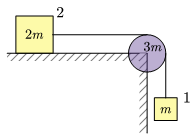
\includegraphics[width=\textwidth]{asset/ch4/T13.png}
    \end{minipage}

    \vspace{-0.5em}
    
    \tcblower
    
    (1)~在本题中，圆盘和两个物体不能视为一个刚体，需要用隔离法分别分析。

    两个物体运动的加速度相同，设为$a$，但要注意两侧绳拉力是不同的。
    
    由牛顿第二定律，$mg-T_1=ma,~T_2=2ma$，根据线量与角量的关系，$a=\alpha R$

    \vspace{0.3em}
    
    对于圆盘，转动惯量为$J=\dfrac{1}{2}3mR^2$，两个力的力臂都是$R$，但方向相反

    \vspace{0.3em}
    
    所以合外力矩$M=(T_1-T_2)R$，代入转动定律得$(T_1-T_2)R=\dfrac{1}{2}\cdot 3mR^2\cdot \alpha$

    \vspace{0.3em}

    联立以上各式解得$a=\dfrac{2}{9}g,~T_1=\dfrac{7}{9}mg,~T_2=\dfrac{4}{9}mg$

    \vspace{0.3em}

    (2)~利用匀变速直线运动规律，$v^2=2ah$. 根据线量和角量的关系，$v=\omega R$，解得$\omega=\dfrac{2\sqrt{2gh}}{3R}$

    \tcbline

    \vspace{-0.5em}
    
    \begin{minipage}{0.85\textwidth}
    【补充练习】半径分别为$R,2R$、质量分别为$m,4m$的均匀圆盘，同轴地粘在一起，可绕过盘心且垂直盘面的水平光滑轴任意转动。两盘边缘都绕有轻绳，下端分别挂有质量均为$m$的物体A、B。求物体A、B运动的加速度。
    \end{minipage}
    \hfill
    \begin{minipage}{0.12\textwidth}
        \centering 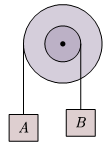
\includegraphics[width=\textwidth]{asset/ch4/T14.png}
    \end{minipage}
    
\end{example}

\section{转动中的功与能}

\subsection{动能定理}

%\subsubsection{力矩做功}

力矩$M$所做的功，就是力矩在角度上的积累。
\begin{formula}
    $W=\displaystyle\int{Fdx}~~~\rightarrow~~~W=\displaystyle\int{Md\theta}$
\end{formula}

%\subsubsection{刚体的转动动能}

绕定轴转动的刚体转动动能可表示为

\begin{formula}
    $E_k=\dfrac{1}{2}mv^2~~~\rightarrow~~~E_k=\dfrac{1}{2}J\omega^2$
\end{formula}

%\subsubsection{动能定理}

合外力矩对定轴转动刚体所做的功，等于转动动能的增量。

\begin{formula}
    $W=\displaystyle\int{Md\theta}=\Delta E_k=\dfrac{1}{2}J\omega_2^2-\dfrac{1}{2}J\omega_1^2$
\end{formula}

%\note{仿照$E_k=\dfrac{1}{2}mv^2$，把$m$替换成$J$，把$v$替换成$\omega$即可。}

\subsection{机械能守恒定律}

\subsubsection{刚体的重力势能}

只要刚体不太大，刚体的重力势能，只需将高度代入质心所在的高度即可。
\begin{formula}
    $E_p=mgh~~~\rightarrow~~~E_p=mgh_C$
\end{formula}

%\note{仿照力的做功，把$F$替换成$M$，把$x$替换成$\theta$即可。}

\subsubsection{守恒定律}

对于包括刚体在内的系统，动能定理、功能原理和机械能守恒定律仍然成立。

如果只有保守内力做功，则系统机械能守恒。

%\note{刚体本身就是一个质点系，所以质点系的动能定理、机械能守恒定律都仍然成立。}

\begin{example}{刚体与机械能守恒}
    \begin{minipage}{0.8\textwidth}
    如图所示，滑轮可视为均匀圆盘，质量为$M$，半径为$R$。在初始状态下，劲度系数为$k$的轻弹簧处于原长，质量为$m$的物体静止于倾角为$\theta$的光滑固定斜面上。求：(1) 重物沿斜面下滑$L$距离后的速度大小；(2) 重物下滑的最远距离。
    \end{minipage}
    \hfill
    \begin{minipage}{0.18\textwidth}
        \centering 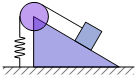
\includegraphics[width=\textwidth]{asset/ch4/T16.png}
    \end{minipage}
    \tcblower

    (1)~在此过程中，只有重力和弹簧弹力做功，系统的机械能守恒。
    
    重力势能转化为弹簧的弹性势能和滑轮与重物的动能，$mgL\sin{\theta}=\dfrac{1}{2}kL^2+\dfrac{1}{2}mv^2+\dfrac{1}{2}J\omega^2$

    \vspace{0.5em}

    均匀圆盘的转动惯量$J=\dfrac{1}{2}MR^2$，根据线量与角量的关系，$v=\omega R$

    \vspace{0.5em}

    联立以上各式解得$v=\sqrt{\dfrac{4mgL\sin\theta-2kL^2}{M+2m}}$

    \vspace{0.5em}
    
    (2)~重物下滑最远距离时，速度为零，重力势能完全转化为弹簧的弹性势能。
    
    \vspace{0.5em}

    由$mgL\sin{\theta}=\dfrac{1}{2}kL^2$，得$L=\dfrac{2mg\sin{\theta}}{k}$
    
    \tcbline

    \vspace{-1em}

    \begin{minipage}{0.8\textwidth}
    【补充练习】长为$L$、质量为$m$的均匀细杆可绕光滑固定轴O在竖直面内旋转，细杆由静止自由下摆，求棒转过$\theta$角时的角速度和角加速度。
    \end{minipage}
    \hfill
    \begin{minipage}{0.18\textwidth}
        
        \centering 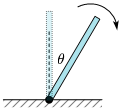
\includegraphics[width=\textwidth]{asset/ch4/T15.png}
    \end{minipage}

    \vspace{-0.5em}
\end{example}

\section{角动量守恒}

\subsection{刚体的角动量}

在质点动力学中，我们已经学习过质点对轴的角动量，等于动量乘以动量臂。

刚体对轴的角动量$L$，等于转动惯量乘以角速度。

\begin{formula}
    $p=mv~~~\rightarrow~~~L=J\omega$
\end{formula}

对于刚体和质点组成的系统，角动量就是系统内所有研究对象的角动量之和。

\subsection{角动量定理}

力矩在时间上的积累称为角冲量或冲量矩$H$，刚体所受角冲量等于角动量的变化$\Delta L$。

\begin{formula}
    $I=\displaystyle \int{Fdt}=\Delta p=p_2-p_1~~~\rightarrow~~~H=\displaystyle \int{Mdt}=\Delta L=L_2-L_1=J\omega_2-J\omega_1$
\end{formula}

\note{动量定理说明冲量等于动量的变化，而角动量定理说明角冲量等于角动量的变化。}

%若考虑刚体和质点组成的系统，则合外力矩的角冲量等于系统角动量的变化，内力矩不产生影响。

\subsection{角动量守恒定律}

对刚体和质点组成的系统，若合外力矩为零，则角动量守恒。

\begin{formula}
    若$M_{\text{外}}=0$，则$L$不变。
\end{formula}

\note{若合外力为零，则动量守恒；若合外力矩为零，则角动量守恒。}

一种常见的情况是，若刚体可绕转轴自由旋转，所受外力全部过转轴，则角动量守恒。

\begin{example}{刚体与角动量守恒}
    \begin{minipage}{0.82\textwidth}
    有半径为$R$、质量为$M$的均匀水平转台，可绕过圆心的转轴自由旋转，中间有一个质量为$m$的人，初始角速度为$\omega_0$，从上向下看为顺时针旋转。
    
    (1)~若人走到转台边缘，并于转台相对静止，求此时的角速度。

    (2)~若人相对圆盘以恒定速率$v$逆时针沿边缘运动，求圆盘的角速度。
    
    \end{minipage}
    \hfill
    \begin{minipage}{0.15\textwidth}
        \centering 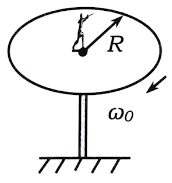
\includegraphics[width=\textwidth]{asset/ch4/T17.png}
    \end{minipage}

    \tcblower

    转台可绕转轴自由旋转，若以人和圆盘组成的系统为研究对象，人与转台之间的力是内力，则所受外力全部过转轴，系统角动量守恒。
    
    (1)~在初状态，人位于圆心，对转动惯量和角动量无贡献。
    
    因此初角动量只需考虑圆盘的贡献，转动惯量$J_1=\dfrac{1}{2}MR^2$，角动量$L_1=J_1\omega_0$

    \vspace{0.5em}
    
    而在末状态，人位于边缘且相对圆盘静止，需要考虑其对转动惯量的贡献。

    \vspace{0.3em}
    
    将人与圆盘视为一个整体，这个整体的转动惯量$J_2=\dfrac{1}{2}MR^2+mR^2$，角动量$L_2=J_2\omega$

    \vspace{0.5em}
    
    根据角动量守恒定律，$L_1=L_2$，解得$\omega=\dfrac{M}{M+2m}\omega_0$

    \vspace{0.5em}

    (2)~在末状态，人和圆盘需要分别计算角动量，系统的角动量是二者之和。

    \vspace{0.3em}
    
    圆盘的转动惯量仍为$J_1=\dfrac{1}{2}MR^2$，角动量为$\dfrac{1}{2}MR^2\omega$

    \vspace{0.5em}

    若以顺时针为正方向，则人相对于大地的速率是$\omega R-v$，因此角动量为$m(\omega R-v)R$

    （回忆第2章质点角动量的知识，匀速圆周运动的质点，其角动量大小为$mvR$）

    \vspace{0.5em}

    根据角动量守恒定律，$L_1=\dfrac{1}{2}MR^2\omega+m(\omega R-v)R$，解得$\omega=\dfrac{MR\omega_0+2mv}{(M+2m)R}$
    
    \tcbline
    \begin{minipage}{0.8\textwidth}
    
    【补充练习】判断下列说法是否正确：(1)~作用力与反作用力的力矩之和为零；(2)~两个等大反向的力作用在刚体上，刚体的角动量不变；(3)~内力矩不改变系统的角动量；(4)~两个相同质量的子弹同时相向射入并留在旋转的盘子内部（如图所示），盘子转动的角速度不变。
    
    \end{minipage}
    \hfill
    \begin{minipage}{0.18\textwidth}
        \centering 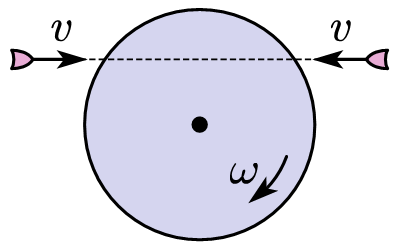
\includegraphics[width=\textwidth]{asset/ch4/T18.png}
    \end{minipage}
    
\end{example}

\subsection{碰撞}

质点的碰撞通常考虑动量守恒，而刚体转动中的碰撞通常考虑角动量守恒。

\note{这是因为在碰撞瞬间，虽然时间极短，但转轴产生的冲击力也很大，不可忽略，所以外力不为零，动量一般不守恒。但是转轴产生的冲击力通过转轴，合外力矩为零，因此碰撞物体构成的系统，角动量守恒。}

\begin{example}{刚体转动与碰撞}
    \begin{minipage}{0.8\textwidth}
    均匀细杆长为$L$，质量为$6m$，被光滑轴固定在天花板上。一个质量为$m$的子弹以速度$v$射入细杆自由端，并留在细杆内。(1)~研究细杆和子弹组成的系统，判断碰撞前后，机械能、动量、对转轴的角动量是否守恒。(2)~求碰撞后瞬间细杆的角速度；(3)~求细杆最大摆角的余弦值。
    
    \end{minipage}
    \hfill
    \begin{minipage}{0.18\textwidth}
        \centering 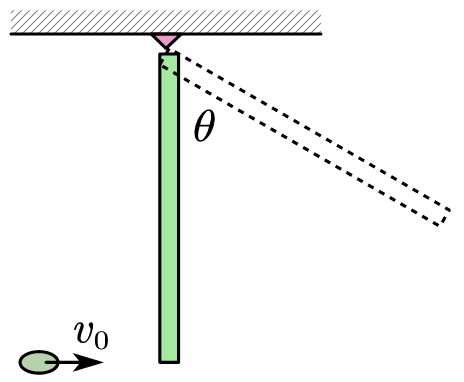
\includegraphics[width=\textwidth]{asset/ch4/T19.png}
    \end{minipage}

    \tcblower
    \setlength{\parskip}{0.1em}

    (1)~由于子弹留在细杆中，相当于完全非弹性碰撞，能量损失最大，机械能不守恒。

    在碰撞瞬间，虽然时间极短，但是转轴处产生的冲击力不可忽略，合外力不为零，动量不守恒。

    但是转轴处产生的冲击力通过转轴，合外力矩为零，所以对转轴的角动量守恒。

    (2)~碰撞前只有子弹在运动，系统角动量$L_1=mvL$

    \vspace{0.3em}

    碰撞后二者结合在一起运动，系统转动惯量$J=\dfrac{1}{3}\cdot 6mL^2+mL^2$，角动量$L_2=J\omega$

    \vspace{0.5em}

    碰撞前后角动量守恒，由$L_1=L_2$解得碰撞后瞬间角速度$\omega=\dfrac{v}{3L}$

    \vspace{0.5em}

    (3)~在碰撞后摆动的过程中，只有重力做功，系统机械能守恒，系统的重力势能可以分别计算。

    \vspace{0.5em}

    由$\dfrac{1}{2}J\omega^2=6mg\dfrac{L}{2}(1-\cos\theta)+mgL(1-\cos\theta)$，求得$\cos\theta=1-\dfrac{3v^2}{8gL}$
    
    \tcbline
    

    \begin{minipage}{0.8\textwidth}
    【补充练习】质量为$m$的黏土块，以水平速度$v$撞在竖直平面的静止圆盘顶端，并粘在一起。圆盘半径为$R$，质量为$2m$，圆盘轴光滑。求：(1)~碰撞后瞬间圆盘的角速度；(2)~圆盘转过$90^\circ$时的角速度。
    
    \end{minipage}
    \hfill
    \begin{minipage}{0.18\textwidth}
        \centering 
\includegraphics[width=\textwidth]{asset/ch4/T20.png}
    \end{minipage}
\end{example}

\subsection{质点与刚体的对比}

\begin{center}
    \begin{tabular}{|c|c|c|}
        \hline
         & 质点 & 刚体 \\
        \hline
        运动的描述 & 线量$x,v,a$ & 角量$\theta, \omega, \alpha$ \\
        \hline
        惯性的度量 & 质量$m$ & 转动惯量$J$ \\
        \hline
        运动定律 & $F=ma$ & $M=J\alpha$ \\
        \hline
        \rule{0pt}{18pt}\rule[-12pt]{0pt}{0pt} 动能 & $E_k=\dfrac{1}{2}mv^2$ & $E_k=\dfrac{1}{2}J\omega^2$ \\
        \hline
        \rule{0pt}{18pt}\rule[-12pt]{0pt}{0pt} 动能定理 & $\displaystyle\int{Fdx}=\Delta E_k$ & $\displaystyle\int{Md\theta}=\Delta E_k$ \\
        \hline
        重力势能 & $E_p=mgh$ & $E_p=mgh_C$ \\
        \hline
        机械能守恒条件 & 只有保守内力做功 & 只有保守内力做功 \\
        \hline
        动量/角动量 & $p=mv$ & $L=J\omega$ \\
        \hline
        \rule{0pt}{18pt}\rule[-12pt]{0pt}{0pt} 动量/角动量定理 & $\displaystyle\int{Fdt}=\Delta p$ & $\displaystyle\int{Mdt}=\Delta L$ \\
        \hline
        动量/角动量守恒条件 & 合外力为零 & 合外力矩为零 \\
        \hline
    \end{tabular}
\end{center}


\section{拓展内容}

\subsection{计算转动惯量的其他方法}

\subsubsection{平行轴定理}

刚体的转动惯量与转轴的选取有关，如果需要平移转轴，可以使用平行轴定理。

若已知转轴过质心的转动惯量$J_C$，将转轴平行移动距离$d$后，转动惯量$J$的公式为
\begin{formula}
    $J=J_C+md^2$
\end{formula}

\warn{注意平行轴定理的基准一定是过质心的转动惯量。}

\subsubsection{正交轴定理}

对于$xy$平面上的薄平板刚体，它对于三个坐标轴的转动惯量满足

\begin{formula}
    $J_z=J_x+J_y$
\end{formula}

例如，以一条直径为轴，圆环的转动惯量$J=\dfrac{1}{2}MR^2$，圆盘的转动惯量$J=\dfrac{1}{4}MR^2$.


\begin{center}
    
\includegraphics[width=0.35\linewidth]{asset/ch4/T21.png}
\end{center}
    
\begin{example}{平行轴定理*}
    如图所示，长为$L$、质量为$m_1$的均匀细杆，一端与转轴相连，另一端连接半径为$r$、质量为$m_2$的均匀圆盘。求整个物体相对于转轴的转动惯量。
    \tcbline

    \begin{minipage}{0.83\textwidth}

    对于细杆而言，转轴位于一端，转动惯量为$\dfrac{1}{3}m_1L^2$

    \vspace{0.3em}

    对于圆盘而言，转轴转轴到圆心的距离是$L+r$，需要使用平行轴定理。

    \vspace{0.3em}
    
    对于过圆心的转轴，转动惯量为$J_0=\dfrac{1}{2}m_2r^2$
    
    \vspace{0.5em}

    利用平行轴定理可知转动惯量变为$\dfrac{1}{2}m_2r^2+m_2(L+r)^2$

    \vspace{0.5em}

    因此整个物体的转动惯量为$J=\dfrac{1}{3}m_1L^2+\dfrac{1}{2}m_2r^2+m_2(L+r)^2$
    \end{minipage}
    \hfill
    \begin{minipage}{0.15\textwidth}
        \centering 
\includegraphics[width=\textwidth]{asset/ch4/T3.png}
    \end{minipage}
    
    \tcblower

    \begin{minipage}{0.69\textwidth}
    【补充练习】三根长为$L$、质量为$m$的均匀细杆焊接成一个等边三角形，转轴垂直于这个三角形所在平面，且过其中一个顶点。求这个物体相对于该转轴的转动惯量。
    \end{minipage}
    \hfill
    \begin{minipage}{0.28\textwidth}
        \centering 
\includegraphics[width=\textwidth]{asset/ch4/T10.png}
    \end{minipage}

\end{example}

\subsection{刚体与质心运动定理}

在刚体转动过程中，若要求出转轴对刚体的力，应考虑使用质心运动定理。

\begin{example}{刚体与质心运动定理结合}
    长为$l$、质量为$m$的均匀细杆，一端用光滑轴固定在天花板上，由水平状态静止下落。求下摆$60^\circ$角时的：(1)~角速度；(2)~角加速度；(3)~转轴对细杆的力。
    \tcblower

    \begin{minipage}{0.73\textwidth}

    (1)~要求角速度应用机械能守恒定律
    
    细杆相对于转轴的转动惯量为$J=\dfrac{1}{3}ml^2$

    \vspace{0.5em}

    注意重心位于细杆中央，因此$\dfrac{1}{2}mgl\sin{60^\circ}=\dfrac{1}{2}J\omega^2$，解得$\omega=\sqrt{\dfrac{3\sqrt{3}g}{2l}}$

    \vspace{0.5em}

    (2)~要求角加速度应用转动定律，$mg\dfrac{l}{2}\cos{60^\circ}=J\alpha$，解得$\alpha=\dfrac{3g}{4l}$
    \end{minipage}
    \hfill
    \begin{minipage}{0.25\textwidth}
        \centering 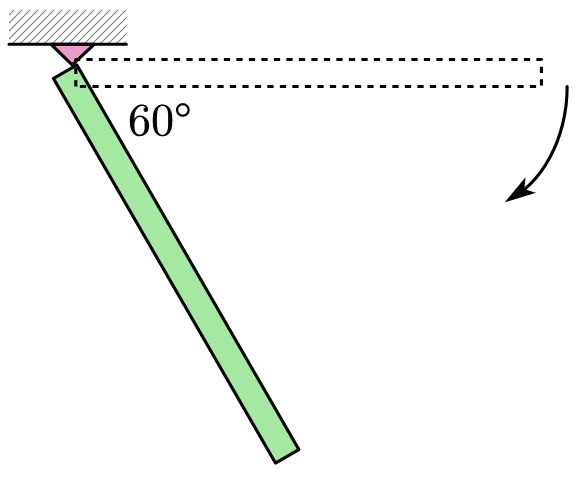
\includegraphics[width=\textwidth]{asset/ch4/T24.png}
    \end{minipage}

    \vspace{0.3em}

    \begin{minipage}{0.78\textwidth}

    (3)~要求转轴对细杆的力，可用质心运动定理。
    
    质心做圆周运动，需要切向和法向分别考虑。

    \vspace{0.3em}

    在沿杆方向上，$F_1-mg\sin{60^\circ}=m\omega^2\dfrac{l}{2}$，得$F_1=\dfrac{5\sqrt{3}}{4}mg$

    \vspace{0.5em}

    在垂直杆方向上，$mg\cos{60^\circ}-F_2=m\alpha\dfrac{l}{2}$，得$F_2=\dfrac{1}{8}mg$
    \end{minipage}
    \hfill
    \begin{minipage}{0.18\textwidth}
        \centering 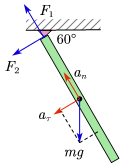
\includegraphics[width=\textwidth]{asset/ch4/T26.png}
    \end{minipage}

    

    \tcbline

    【补充练习】针对补充练习7的情景，在圆盘转过$90^\circ$时，求：(1)~圆盘转动的角加速度；(2)~转轴对圆盘的作用力。
\end{example}



\subsection{平面运动的刚体}

\noindent
\begin{minipage}{0.83\textwidth}
\setlength{\parindent}{2em}
\setlength{\parskip}{0.5em}
\linespread{1.3}

    对于做平面运动的刚体，其运动可以分解为整体随质心的平动和绕质心的转动。

    根据柯尼希定理，刚体的动能就等于这两项动能之和。
    
    \begin{formula}
        $E_k=\dfrac{1}{2}mv_C^2+\dfrac{1}{2}J\omega_C^2$
    \end{formula}
    
    \end{minipage}
    \hfill
    \begin{minipage}{0.15\textwidth}
        \centering 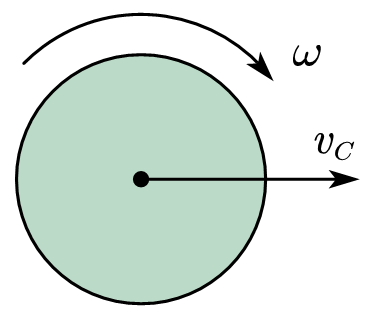
\includegraphics[width=\textwidth]{asset/ch4/T25.png}
    \end{minipage}

\begin{example}{平面运动的刚体*}
    长为$L$的均匀细杆竖直放在光滑地面上，从静止倒下，求杆滑到地面瞬间的质心速度。
    \tcblower
    
    \begin{minipage}{0.73\textwidth}

    杆在水平方向不受外力，因此质心速度一定竖直向下，设为$v$

    杆的A端在水平面上运动，在最终状态运动到最远点，速度为零。

    \vspace{0.3em}

    因此杆绕质心转动的角速度$\omega$满足$v=\omega \cdot \dfrac{L}{2}$

    \vspace{0.5em}
    
    整个过程只有重力做功，机械能守恒，$mg\dfrac{L}{2}=\dfrac{1}{2}mv^2+\dfrac{1}{2}J\omega^2$

    \vspace{0.5em}

    其中杆绕质心的转动惯量$J=\dfrac{1}{12}mL^2$，联立解得$v=\dfrac{\sqrt{3gL}}{2}$.
    \end{minipage}
    \hfill
    \begin{minipage}{0.25\textwidth}
        \centering 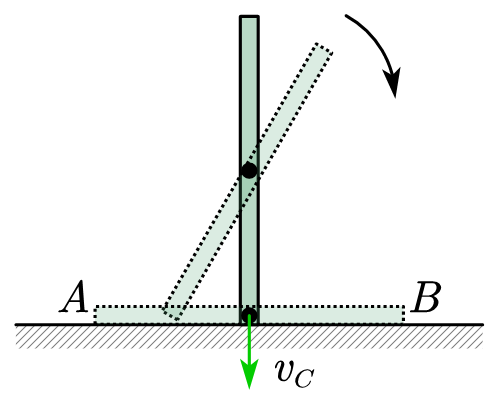
\includegraphics[width=\textwidth]{asset/ch4/T22.png}
    \end{minipage}
    
    \tcbline
    \begin{minipage}{0.82\textwidth}
    【补充练习】半径为$R$、质量为$m$的匀质实心球由静止沿斜面无滑动地滚动下来，求质心下降$h$时的速度大小。
    \end{minipage}
    \hfill
    \begin{minipage}{0.15\textwidth}
        %\vspace{-2em}
        \centering 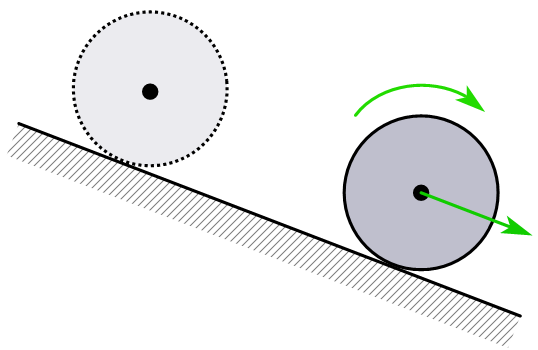
\includegraphics[width=\textwidth]{asset/ch4/T23.png}
    \end{minipage}
    
\end{example}

\subsection{连续受力的刚体}

\begin{example}{连续受力的刚体}
    长为$L$、质量为$m$的均匀细杆放在桌面上，绕中点在桌面上旋转。桌面与细杆的动摩擦因数为$\mu$. 求：(1) 细杆所受的摩擦力矩；(2) 细杆转动的角加速度。
    \tcblower
    (1)~将细杆切成长为$dx$的小段，每小段的质量为$m\dfrac{dx}{L}$，所受摩擦力为$\mu mg\dfrac{dx}{L}$
    
    对于到中点距离为$x$的小段，摩擦力矩为$\mu mg\dfrac{xdx}{L}$

    因此全长的摩擦力矩为$M=2\displaystyle\int_0^{L/2}{\mu mg\dfrac{xdx}{L}}=\dfrac{\mu mgL}{4}$

    (2)~细杆相对于中点的转动惯量为$J=\dfrac{1}{12}mL^2$，根据转动定律$M=J\alpha$，可得$\alpha=\dfrac{3\mu g}{L}$

    \tcbline

    【补充练习】半径为$R$、质量为$m$的均匀圆盘放在桌面上，绕圆心在桌面上旋转。桌面与圆盘的动摩擦因数为$\mu$. 若圆盘的初角速度为$\omega$，求停止之前转过的角度。
\end{example}